\documentclass[12pt]{article}

\usepackage{sbc-template}
\usepackage{textcomp}
\usepackage{listings}
\usepackage{graphicx,url}
\usepackage{framed}
\usepackage{color}
\usepackage[utf8]{inputenc}
\usepackage{fontenc}

\renewcommand\lstlistingname{Listagem}
\renewcommand\lstlistlistingname{Lista de Listagens}
\renewcommand\figurename{Imagem}
\renewcommand\listfigurename{Lista de Imagens}
\renewcommand\tablename{Tabela}
\renewcommand\listtablename{Lista de Tabelas}

% Definição do template de formatação e synthax hightlight para groovy :)
%
\lstdefinelanguage{Groovy}{keywords={
                                            abstract, default, if, private, this,
                                            boolean, do, implements, protected, 
                                            throw, break, double, import, public, 
                                            throws, byte, else, instanceof, return,
                                            transient, case, extends, int, short, 
                                            try, catch, final, interface, static, 
                                            void, char, finally, long, strictfp,
                                            volatile, class, float, native, super, 
                                            while, const, for, new, switch, continue,
                                            goto, package, synchronized, def, any, 
                                            as, in, with, null, true, false, static
                                },
                                keywords={[2]params, render,it, flash, redirect},
                                morecomment=[l]{//},
                                morecomment=[s]{/*}{*/},
                                morestring=[b]",
                                morestring=[d]',
                                morestring=[b]""",
                                morestring=[b]''',
                                morestring=[b]/
                           }

%
%   Definição de estilos das linguagens
%
%\lstdefinestyle{Listagem}{
%                        \lstlistingname
%                        }
\lstdefinestyle{Groovy}{
                            upquote=true,
                            basicstyle=\small,
                            keywordstyle=\color[RGB]{151,40,120},
                            keywordstyle={[2]\color[RGB]{102, 204, 255}},
                            stringstyle={\color[RGB]{255,0,204}
                                         \ttfamily
                                         \small
                            },
                            identifierstyle=\ttfamily,
                            breaklines=true,
                            showtabs=false,
                            showspaces=false,
                            showstringspaces=false,
                            columns=fullflexible,
                            numbers=left,
                            language=Groovy,
                            name=Listagem
                            extendedchars=true,
                            frame=leftline
                       }
\lstdefinestyle{InlineGroovy}{
                           style=Groovy,
                           numbers=none
                      }
\lstdefinestyle{Java}{
                        keywordstyle={\color[RGB]{127,0,85} \ttfamily \small },
                        stringstyle={\color[RGB]{42,0,255} \ttfamily \small},
                        commentstyle={\color[RGB]{63,127,95} \ttfamily \small},
                        upquote=true,
                        basicstyle=\small,
                        breaklines=true,
                        showtabs=false,
                        showspaces=false,
                        showstringspaces=false,
                        columns=fullflexible,
                        numbers=left,
                        language=Java,
                        name=Listagem,
                        frame=leftline                   
                     }
\hyphenation{chave/valor}
\sloppy

\title{Groovy on Rails, uma alternativa para o desenvolvimento de aplicações web
       sem sair da Plataforma Java}

\author{Marcelo Emanoel Bezerra Diniz\inst{1}}

\address{
    Centro de Ciências Tecnológicas -- Universidade de Fortaleza (UNIFOR)\\
    CEP 60.811-905 -- Fortaleza -- CE -- Brasil
}

\begin{document} 

\maketitle

\begin{resumo} 
    
    Desde seu surgimento a plataforma Java se destaca como uma ótima alternativa
    para o desenvolvimento de aplicações web. Diversos frameworks surgiram para 
    proporcionar reutilização de código e aumento de produtividade. A plataforma
    possui implementações robustas e amplamente utilizadas. Porém, apesar dos 
    esforços, outras tecnologias mais recentes vêm se destacando e tomando a 
    frente no cenário de desenvolvimento de aplicações para a web. Dentre estas 
    tecnologias são notórias algumas características como o uso de linguagens 
    dinâmicas em conjunto com padrões de projeto amplamente conhecidos. Neste 
    artigo será abordado o framework Groovy on Rails, ou simplesmente Grails. 
    O framework alia a linguagem dinâmica Groovy à arquitetura utilizada no Ruby 
    on Rails. \nocite{*}
    
\end{resumo}

\section{Introdução}

    Alta competitividade, baixo custo de produção e manutenção, além de alta 
    qualidade, são exigências do mercado de desenvolvimento de software. 
    Independentemente da tecnologia envolvida no processo de construção de uma 
    aplicação web, existe o componente de complexidade inerente ao próprio 
    ambiente. Toda a comunicação é baseada no protocolo HTTP. Sua simplicidade 
    garante a alta disponibilidade da web, porém requer um trabalho adicional 
    das aplicações para manter as informações seguras e íntegras.

    No cenário previamente descrito, a plataforma Java se destacou desde o seu 
    sur\-gi\-men\-to. A fim de facilitar o desenvolvimento das aplicações para este 
    ambiente, surgiram diversos frameworks, bases de infra-estruturas 
    extensíveis, voltadas para um nicho em particular. A partir destas o 
    desenvolvedor irá retirar os insumos para a construção de aplicações.

    Com o passar do tempo, outras linguagens dentro e fora da plataforma foram 
    surgindo com propostas um pouco diferentes da linguagem Java. Algumas com 
    características funcionais, outras com características totalmente orientadas 
    a objetos, porém, todas com um foco em comum, aumento de produtividade, 
    possibilitando entregar mais funcionalidades com menos código. Em cima 
    dessas novas linguagens, novos frameworks foram sendo desenvolvidos para 
    resolver de forma melhor os antigos problemas.
    
    Nesse cenário, em julho de 2004, surgiu o framework Ruby on Rails 
    para a linguagem Ruby. Suas bases advêm do padrão de projeto arquitetural MVC. 
    Voltado para o desenvolvimento de aplicações web, rapidamente adquiriu adeptos por 
    facilitar e agilizar a criação de aplicações através de geradores de código 
    para as tarefas comuns, além, é claro, da utilização de uma linguagem de mais 
    fácil compreensão.

    Com a popularização desse conjunto de novas linguagens, implementações 
    baseadas na Java Virtual Machine, JVM, foram surgindo. Através da JSR, Java 
    Specification Request, número 223, a integração de linguagens de script foi 
    facilitada. Nesse contexto uma nova linguagem surgiu, Groovy. Sua plataforma 
    única é a JVM, isso significa que o compilador da linguagem produz o mesmo
    bytecode gerado pelo compilador Java. E que portanto, automaticamente um 
    extenso conjunto de bibliotecas pré-existentes e maduras pode ser utilizado 
    na nova linguagem de maneira transparente para o desenvolvedor. 
    
    Com a popularização do Ruby on Rails muitas de suas funcionalidades foram 
    incorporadas por alguns frameworks mesmo que em outras linguagens. A 
    abordagem utilizada no Groovy on Rails, Grails, possui algumas similaridades 
    e algumas diferenças. Seu foco está em utilizar fórmulas consagradas na 
    Plataforma Java e aliar às inovações do Rails produzindo um ambiente de alta 
    produtividade utilizando soluções maduras.
    
    Nas seções seguintes serão descritos os principais conceitos da linguagem 
    Groovy e do framework Grails.

\section{A linguagem Groovy} \label{sec:linguagem_groovy}

    A linguagem Groovy, criada em  Agosto de 2003, é dinamicamente tipada e pode
    ser interpretada ou compilada. Foi elaborada para ser executada especificamente
    pela JVM e sofreu grande influência das linguagens Ruby, Python, Perl, 
    Smalltalk e, obviamente, de Java.
    
    A elaboração da linguagem Groovy com a JVM como plataforma principal permitiu 
    que pouca ou nenhuma distorção possa existir entre as linguagens, além disso, 
    esta escolha reduziu de maneira drástica a curva de aprendizado. Sua API, 
    \emph{Application Programming Interface} (Interface de Programação de Aplicações), 
    é toda baseada na API Java padrão; aliado a isto, a integração com a JVM no 
    nível de \emph{bytecode} permite a interoperabilidade de Java para Groovy bem como 
    o caminho reverso. Dessa maneira, desenvolvedores Java automaticamente também 
    desenvolvem em Groovy.
    
    Dentre as funcionalidades que a linguagem possui é possível citar o uso de 
    \emph{closures},  e propriedades nativas bem como a utilização de metaprogramação, 
    que como consequência direta proporciona a criação das chamadas \emph{Domain 
    Specific Languages} ou simplesmente DSL's.

\subsection{Instalação}
    
    No endereço \url{http://groovy.codehaus.org/Download} é possível fazer o 
    download das ferramentas necessárias à utilização da linguagem. Lá é possível
    encontrar instaladores para as plataformas Windows e Debian bem como a versão
    binária que pode ser usada em qualquer sistema operacional. Para o Mac OS X 
    é possível utilizar algum dos gerenciadores de pacotes existentes como o 
    Macports ou o Homebrew.

    Após a instalação do Groovy deve ser possível agora executar no console os comandos:
    
    \begin{description}
        \item [groovysh:] Abre o Groovy Shell
        \item [groovyConsole:] Abre o console gráfico do Groovy 
        \item [groovy:] Executa um arquivo groovy
        \item [groovyc:] Compila um arquivo .groovy em .class
    \end{description}
    
\subsection{Groovy Script}
    
    Como dito anteriormente, Groovy pode ser utilizado como uma linguagem de 
    script para execução de tarefas rápidas. Para exemplificar, veremos o clássico
    exemplo HelloWorld utilizando Groovy como script. A listagem \ref{HelloGroovyScript}
    mostra o conteúdo do arquivo Hello.groovy. 
    
    \lstinputlisting[   
                        style=Groovy,
                        caption=Hello World Groovy Script,
                        label=HelloGroovyScript
                    ]
                    {src/groovy/Hello.groovy}

    Executando o comando:
    \begin{lstlisting}[basicstyle={\small \ttfamily}]
        groovy Hello.groovy
    \end{lstlisting}
    
    O resultado, como esperado, é que no console o texto "Hello Groovy Script World"
    seja impresso. Isso acontece por que o interpretador internamente cria um 
    método \texttt{main} e insere o código contido no arquivo \texttt{Hello.groovy}.
    O código Java equivalente pode ser observado na listagem \ref{HelloGroovyScriptInJava}.
    
    \lstinputlisting[
                        style=Java,
                        caption=Hello World Groovy Script em Java,
                        label=HelloGroovyScriptInJava
                    ]
                    {src/java/Hello.java}

\subsubsection{Funções de Script}

    Assim como outras linguagens de script é possível criar blocos de código 
    reutilizáveis, as funções. A listagem \ref{HelloGroovyScriptWithFunctions} 
    fornece um exemplo da sintaxe utilizada para a declaração de funções.
    
    \lstinputlisting[
                        style=Groovy,
                        caption=Hello World Groovy Script Com Funções,
                        label=HelloGroovyScriptWithFunctions,
                    ]
                    {src/groovy/HelloWithFunctions.groovy}
   

\subsection{Strings}

    Strings em Groovy podem ser definidas de até cinco formas diferentes, são elas:
    
    \begin{enumerate}
        \item entre aspas duplas: 
            \begin{lstlisting}[style=InlineGroovy]
                "Marcelo Emanoel"
            \end{lstlisting}
        \item entre aspas simples:
            \begin{lstlisting}[style=InlineGroovy]
                'Marcelo Emanoel'
            \end{lstlisting}
        \item entre barras:
            \begin{lstlisting}[style=InlineGroovy]
                /Marcelo Emanoel/
            \end{lstlisting}
        \item entre três aspas duplas: 
            \begin{lstlisting}[style=InlineGroovy]
                """Marcelo Emanoel"""
            \end{lstlisting}
        \item entre três aspas simples:
            \begin{lstlisting}[style=InlineGroovy]
                '''Marcelo Emanoel'''
            \end{lstlisting}

    \end{enumerate}
    
    A depender da forma declarada é possível que a string produzida aceite ou não
    o uso de interpolação, ou seja, a inserção de expressões que serão avaliadas
    e concatenadas à string. A listagem \ref{HelloGroovyScriptWithFunctions} exibe
    este conceito na linha 2 onde o resultado da expressão deli\-mitada por \$\{ e \}
    é concatenado à string. A listagem \ref{HelloGroovyScriptWithFunctionsInJava}
    exibe o código Java equivalente.
    
    \lstinputlisting[
                        style=Java,
                        caption=Hello World Groovy Script Com Funções Em Java,
                        label=HelloGroovyScriptWithFunctionsInJava
                    ]
                    {src/java/HelloWithFunctions.java}

    Dentre as formas descritas anteriormente apenas as seguintes aceitam 
    interpolação: 1, 3 e 4. O resultado da tentativa de utilização da técnica com
    os outros tipos de declarações de string resulta na concatenação da expressão
    não avaliada, ou seja, a própria expressão. Como por exemplo \textbf{\$\{name\}}
    na string final. 

    Os tipos 4 e 5 citados anteriormente produzem um tipo especial de string que
    pode ser expandido por mais de uma linha, por isso são chamados de \emph{multilinhas}.
    Uma utilização prática e direta da interpolação de strings em conjunto com as
    strings \emph{multili\-nhas} é a criação de \emph{templates} de forma transparente. 
    
    Como dito anteriormente, uma outra forma de declarar uma string é inserindo
    conteúdo entre \emph{/}. Esse tipo de declaração permite criar valores sem 
    ter que utilizar ca\-racteres de escape para símbolos especiais com exceção 
    do próprio \emph{/}. Assim, é possível simplificar por exemplo a escrita de 
    expressões regulares como mostra a listagem \ref{SlashyStringWithRegex}.
    
    \lstinputlisting[
                        style=Groovy,
                        caption=Simplificação de Expressões Regulares com Slashy 
                                Strings,
                        label=SlashyStringWithRegex
                    ]
                    {src/groovy/SlashyStringWithRegex.groovy}

\subsection{Métodos e Closures}

    A linguagem possibilita duas formas de estruturação de blocos de código 
    reutilizáveis. Métodos e Closures. A sintaxe de definição de métodos
    é bastante simples e já foi vista nos exemplos anteriores. É necessário apenas
    que se façam alguns esclarecimentos sobre métodos:

    \begin{enumerate}
        \item O tipo de retorno do método bem como a palavra chave \emph{return}
              são opcionais. Por padrão o resultado da avaliação da última linha
              do método é retornada.
        \item Por padrão, propriedades, métodos e classes são públicos. Para alterar
              este comportamento basta utilizar o modificador de acesso correspondente
              para a visibilidade pretendida.
        \item É possível definir parâmetros com valores padrão. Isso possibilita
              que o mesmo método possa ser chamado de diferentes formas. A listagem
              \ref{MethodWithDefaultParameters} exemplifica a sintaxe da declaração.
    \end{enumerate}
    
    \lstinputlisting[
                        style=Groovy,
                        caption=Método com parâmetros com valores padrão,
                        label=MethodWithDefaultParameters
                    ]
                    {src/groovy/MethodWithDefaultParameters.groovy}

\subsection{Closures}

    Closures são pedaços de código reutilizáveis que possuem escopo e podem ser 
    retornados a partir de métodos, atribuídos a propriedades ou variáveis e 
    ainda podem ser utilizados como argumentos em uma chamada de método. 
    
    Estruturas representadas através da notação \{ ... \} representam closures.
    O código dentro das chaves é executado sempre que a closure é invocada, 
    funcionando de maneira similar aos métodos, podem inclusive ter parâmetros. 
    A diferença básica entre os dois é que as primeiras são objetos enquanto os 
    últimos não. A listagem \ref{HelloClosures} exemplifica a construção de uma 
    closure e sua execução.
    
    \lstinputlisting[
                        style=Groovy,
                        caption=Exemplo de definição e chamada de closures,
                        label=HelloClosures,
                        escapeinside=-+
                    ]
                    {src/groovy/HelloClosures.groovy}
    
\subsection{Collections}

    Groovy possui vários tipos de coleções incluindo listas, mapas, conjuntos,
    \texttt{arrays} e intervalos. Neste artigo, apenas listas e mapas serão explicados.
    
\subsubsection{Listas}

    Assim como em Java, uma lista em Groovy é uma coleção ordernada de objetos e 
    implementam a interface \emph{java.util.List}. Sua sintaxe de declaração é 
    semelhante à de \texttt{arrays} como pode ser visto na Listagem \ref{GroovyLists}.
    
    \lstinputlisting[
                        style=Groovy,
                        caption=Listas,
                        label=GroovyLists
                    ]
                    {src/groovy/GroovyLists.groovy}

\subsubsection{Mapas}

    Assim como em Java, um mapa em Groovy é uma coleção não ordenada de pares 
    chave/valor onde as chaves são únicas. Os mapas seguem a interface \emph{java.util.Map}
    e têm como implementação padrão utilizada a classe \emph{java.util.LinkedHashMap}.
    Entretanto, é possível utilizar outras implementações bastando apenas inicializar
    a variável com o tipo desejado.
    
    De maneira semelhante às listas os mapas podem ser declarados com a notação
    de arrays onde as chaves não são números. A listagem \ref{GroovyMaps} exemplifica
    a utilização de mapas.
    
    \lstinputlisting[  
                        style=Groovy,
                        caption=Mapas,
                        label=GroovyMaps
                    ]
                    {src/groovy/GroovyMaps.groovy}
    
\subsection{Redefinição de Operadores}  
    
    Assim como em algumas linguagens, como C++ e Ruby, é possível redefinir operadores.
    Para tanto, Groovy se utiliza de métodos com assinaturas pré-definidas nas classes.
    Assim, é possível, por exemplo, fazer com que dois objetos do tipo \texttt{BigDecimal}
    possam ser adicionados utilizando o operador de adição +. A tabela 
    \ref{tab:OperatorDefinition}, retirada do cartão de referência de \cite{groovy:refcard} 
    exibe os métodos que precisam ser definidos para a utilização dos respectivos 
    operadores.

    \begin{table}[h]
        \centering
        \caption{Sobrescrita de Operadores}
        \label{tab:OperatorDefinition}
        \begin{tabular}{| c | c | c | c |}
        \hline
        {\bf Operador} & {\bf Método} & {\bf Operador} & {\bf Método} \\
        \hline
             a + b &  a.plus(b) & a - b & a.minus(b) \\
        \hline
             a * b & a.multiply(b) & a / b &   a.div(b) \\
        \hline
            a \% b &   a.mod(b) &  a ** b & a.power(b) \\
        \hline
            a \texttt{|} b & a.or(b) & a \texttt{\&} b & a.and(b) \\
        \hline
            a \texttt{\^} b & a.xor(b) & \texttt{\~}a & a.bitwiseNegate() \\
        \hline
            a+ & a.postive() & -a & a.negative() \\
        \hline
            a[b] & a.get(b) & a[b] = c & a.putAt(b, c) \\
        \hline
            a \texttt{<<} b & a.leftShift(b) & a \texttt{>>} b & a.rightShift(b)\\ 
        \hline
            a \texttt{>>>} b & a.rightShiftUnsigned(b) & switch(a) \{case(b) : ... \} & b.isCase(a) \\
        \hline
            a == b & a.equals(b) & a != b & !a.equals(b) \\
        \hline
           a \texttt{<=>} b & a.compareTo(b) & a \texttt{>} b & a.compareTo(b) \texttt{>} 0 \\
        \hline
            a \texttt{>=} b & a.compareTo(b) \texttt{>=} 0 & a \texttt{<} b & a.compareTo(b) \texttt{<} 0 \\
        \hline
            a \texttt{<=} b & a.compareTo(b) \texttt{<= 0} & a as b & a.asType(B) \\
        \hline
            a++ & \multicolumn{ 1}{|c|}{a.next()} & a- - & \multicolumn{ 1}{|c|}{a.previous()} \\
            ++a & \multicolumn{ 1}{|c|}{} & - -a & \multicolumn{ 1}{|c|}{} \\
        \hline
        \end{tabular}  
    \end{table}

\subsection{Operadores Especiais}

    Além dos operadores exibidos na tabela \ref{tab:OperatorDefinition} Groovy 
    oferece outros específicos.

\subsubsection{Operador Elvis}

    De acordo com \cite{beginingGroovy:2008} o operador \texttt{elvis} (\texttt{?:}) é equivalente
    ao operador de \texttt{if} ternário em Java, como demonstra a listagem \ref{ternaryIfJava}.
    Em Groovy o operador \texttt{elvis} permite a escrita de maneira ainda mais concisa 
    como pode ser visto na listagem \ref{elvisOperatorGroovy} com o código equivalente.
    
    \lstinputlisting[
                        style=Java,
                        caption=Funcionamento do If Ternário em Java,
                        label=ternaryIfJava
                    ]
                    {src/java/TernaryIfJava.java}
    
    \lstinputlisting[
                        style=Groovy,
                        caption=Funcionamento do Operador Elvis,
                        label=elvisOperatorGroovy,
                        escapeinside=-+
                    ]
                    {src/groovy/ElvisOperator.groovy}
                    
\subsubsection{Operador Spread}

    O operador de \emph{spread} (\texttt{*.}) como explicado na seção de operadores
    especiais do livro \emph{Beginning Groovy and Grails From Novice to Professional}
    \cite{beginingGroovy:2008} permite que uma operação seja realizada nos itens 
    de uma coleção de maneira mais sucinta. A listagem \ref{SpreadOperator} 
    reproduz o trecho de código na seção 2-35 do livro citado no início do parágrafo 
    exemplificando duas maneiras de iterar numa lista, através da \emph{closure} 
    \texttt{collect()} e do operador de \emph{spread}.
    
    \lstinputlisting[
                        style=Groovy,
                        caption=Listagem 2-35 do livro Beginning Groovy and Grails From Novice to Professional,
                        label=SpreadOperator
                    ]
                    {src/groovy/SpreadOperator.groovy}

% iniciar uma subseção e falar sobre o básico da linguagem
% incluir:
%    shell/console + definição de funções -> DONE
%    Strings: multiline, interpolation -> DONE
%    métodos -> DONE
%    closures -> DONE
%    básico de collections:
%       listas -> DONE
%       mapas -> DONE
%    operators 
%       overloading -> DONE
%       elvis operator -> DONE
%       spread operator -> DONE
%

\section{Grails Framework}
\hyphenation{e-xis-te scaffold scaffol-ding}
    O framework é focado no desenvolvimento rápido de aplicações web. Utiliza como
    base tecnologias consagradas como Spring, Hibernate e Sitemesh. Se baseia 
    fortemente nos princípios de convenções sobre configurações, mapeamento objeto
    relacional, \emph{plugins}, \emph{scaffolding} e testes unitários \cite{beginingGroovy:2008}.
    Pelo fato de ter Groovy como base existe ainda a integração em nível de \emph{bytecode},
    além disso, uma aplicação Grails pode ser empacodata em um arquivo WAR, o que 
    possibilita a implantação em qualquer servidor de aplicações JEE ou qualquer
    container web como é o caso do Jetty (\url{http://jetty.codehaus.org/jetty/})
    ou o Tomcat (\url{http://tomcat.apache.org/download-70.cgi}).
    
\subsection{Instalação}
    
    O framework, assim como o Groovy, tem como requisito o Java SDK versão 5.0 ou 
    superior com a variável de ambiente \texttt{JAVA\_HOME} devidamente instalada 
    e apontando para o diretório de instalação do SDK. 
    
    De acordo com \cite{grails} os passos para a instalação do Grails são os seguintes:
    \begin{enumerate}
        \item Efetuar o download da última versão do Grails, atualmente 1.3.7, e extrair
              para um local apropriado.
        \item Criar uma variável de ambiente chamada \texttt{GRAILS\_HOME} apontando para
              o diretório escolhido no passo anterior.
        \item Adicionar ao \texttt{PATH} do sistema o caminho \texttt{GRAILS\_HOME/bin}.
    \end{enumerate}

    Com todos os passos executados resta abrir um terminal e executar o comando 
    \emph{grails}. Caso uma mensagem de ajuda seja exibida tudo está funcionando corretamente. 

    Alguns sistemas operacionais possuem pacotes de instalação prontos como o Mac
    OS X e o Ubuntu. Para usuários do Mac OS X com o Homebrew instalado basta executar
    no terminal o comando \emph{brew install grails} e, ao término, tudo deve 
    estar funcionando. Já para quem utiliza o Ubuntu é possível utilizar o comando 
    \emph{apt-get} a partir dos seguintes passos:
    
    \begin{enumerate}
        \item sudo add-apt-repository ppa:groovy-dev/grails
        \item sudo apt-get update
        \item sudo apt-get install grails
    \end{enumerate}

\subsection{Primeira Aplicação Grails: Agenda de Contatos}

    A fim de entender o funcionamento do framework será criada uma aplicação web
    que vai explorar de uma maneira mais dinâmica as principais funcionalidades
    oferecidas.
%    listar todos os contatos -> DONE
%    listar os contatos agrupados -> 
%    adicionar grupos -> DONE
%    associar contatos a um grupo -> DONE
%    exibir, editar, salvar e apagar contatos e grupos -> DONE

    A aplicação é uma \textbf{agenda de contatos} onde cada \textbf{contato} pode 
    pertencer a um ou mais \textbf{grupos}. Cada \textbf{contato} pode possuir foto,
    endereços de e-mail e físico, telefone(s), url de site, endereço de perfil no 
    Google etc. Na aplicação é possível \emph{listar todos os \textbf{contatos}}, 
    \emph{listar os \textbf{contatos} agrupados}, \emph{adicionar \textbf{grupos}}, 
    \emph{associar \textbf{contatos} a um \textbf{grupo}} e \emph{exibir}, 
    \emph{editar}, \emph{salvar} e \emph{apagar} \textbf{contatos e grupos}.
    
    A primeira atividade necessária é criar a aplicação, para isso é necessário
    digitar no console/terminal o seguinte comando:
    
    \begin{lstlisting}[basicstyle={\small \ttfamily}]
        grails create-app agenda
    \end{lstlisting}
    
    Isso irá acionar o grails e ele irá criar toda a estrutura inicial necessária para
    o funcionamento do projeto. A partir deste momento a aplicação já pode ser 
    executada. Para tanto entre no diretório criado e digite o comando:
    
    \begin{lstlisting}[basicstyle={\small \ttfamily}]
        grails run-app
    \end{lstlisting}
    
    Imediatamente uma instância do container web \emph{Tomcat} será criada e estará a
    espera de conexões na porta 8080 por padrão. Para testar se a aplicação está
    sendo executada é possível acessar o endereço \url{http://localhost:8080/agenda} 
    e o resultado deve ser semelhante ao da imagem \ref{fig:firstRun}
    
    \begin{figure}[h!]
    \centering
    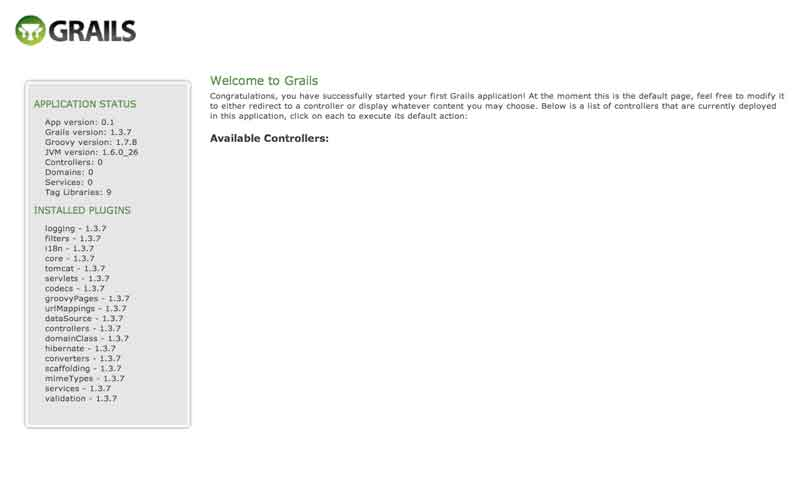
\includegraphics[width=0.8\textwidth]{images/firstRun.jpg}
    \caption{Primeira execução da aplicação Agenda}
    \label{fig:firstRun}
    \end{figure}
    
    O script de criação da aplicação criou a estrutura de diretórios que pode ser
    visualizada na imagem \ref{fig:appStructure} e descrita na tabela \ref{tab:appStructure}.
    
     \begin{table}[h]
          \centering
          \caption{Sobrescrita de Operadores}
          \label{tab:appStructure}
          \begin{tabular}{| l | l |}
          \hline
          {\bf Diretório} & {\bf Descrição} \\
          \hline
              grails-app & Diretório principal da aplicação \\
          \hline
               grails-app/conf & Contém os arquivos de configuração da aplicação \\
          \hline
              grails-app/controllers &  Contém todas os controllers da aplicação, \\
                                     & corresponde ao C do MVC\\
          \hline
              grails-app/domain & Contém as entidades da aplicação, são automaticamente\\
                                & persistentes, corresponde ao M do MVC \\
          \hline
              grails-app/i18n & Contém os arquivos properties utilizados na internacionalização \\
          \hline
              grails-app/services  & Contém as classes de services, são beans do Spring \\
          \hline
              grails-app/taglib & Contém os arquivos de tags customizadas para utilização \\
                                & nas views escritas com Groovy Server Pages (GSP) \\
          \hline
              grails-app/utils & Contém utilitários específicos do Grails \\ 
          \hline
              grails-app/views & Contém todos os arquivos GSP da aplicação, corresponde \\
                               & ao V do MVC \\
          \hline
              lib & Contém todos os arquivos .jar externos que são necessários a\\
                  &  aplicação como por exemplos drivers JDBC \\
          \hline
              scripts & Contém scripts customizados para utilização na aplicação \\
          \hline
              src & Contém diretórios groovy e java com código fonte que \\
                  & estarão disponíveis para aplicação em tempo de execução \\
          \hline
              target & Contém todos os arquivos binários da aplicação \\
          \hline
              test & Contém diretórios para testes de unidade e de integração\\
          \hline
          \end{tabular}  
      \end{table}
    
    \begin{figure}[h!]
    \centering
    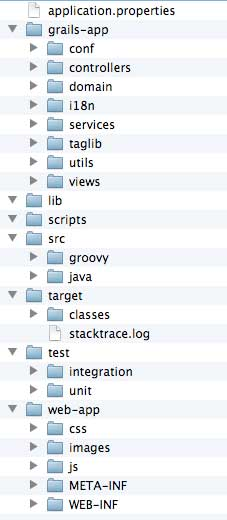
\includegraphics[width=.25\textwidth]{images/appStructure.jpg}
    \caption{Estrutura de pastas e arquivos criadas}
    \label{fig:appStructure}
    \end{figure}

\subsection{Criando Domain Classes - Os Contatos da Aplicação}

    Segundo \cite{pragmaticGrails:2009} o coração do \emph{Grails} está nas \emph{Domain Classes}.
    Elas são classes que representam o domínio do negócio, seus relacionamentos e
    são persistentes. Existe a convenção que uma \emph{Domain Class} está diretamente 
    ligada a uma tabela em um banco de dados.
    
    Agora que já se sabe o que é, é possível criar a primeira classe do sistema 
    de contatos. A classe Contato, que representa um contato. Um contato no sistema
    possui os seguintes atributos:
    
    \begin{description}
        \item[nome:] Representa o nome do contato;
        \item[email:] Representa o email do contato;
    \end{description}
    
    Para a criar uma classe de domínio utiliza-se o comando: 

    \begin{lstlisting}[basicstyle={\small \ttfamily}]
       grails create-domain-class <[pacote.]NomeDaClasse>
    \end{lstlisting}
    
    onde:
    
    \begin{description}
        \item[pacote:] é opcional e representa o nome do pacote que a classe 
                      pertencerá, caso não informado, tem por valor padrão o nome
                      da aplicação;
        \item[NomeDaClasse:] é obrigatório e representa o nome da classe que será
                             criada.
    \end{description}
    
    Assim, para criar a classe Contato devemos executar o comando:
    
    \begin{lstlisting}[basicstyle={\small \ttfamily}]
        grails create-domain-class agenda.Contato
    \end{lstlisting}
    
    Com isto o framework cria uma classe chamada \texttt{Contato} dentro do pacote agenda 
    e um teste unitário chamado \texttt{ContatoTest} também dentro do pacote agenda.
    
    O resultado final incluindo as propriedades inseridas manualmente pode ser visto
    nas listagens \ref{ContactV1} e \ref{ContactTestV1} a seguir.
    
    \lstinputlisting[
                      style=Groovy,
                      caption=Domain Class Contato com propriedades name e email,
                      label=ContactV1
                    ]
                    {src/groovy/agenda/contato/ContatoV1.groovy}

   \lstinputlisting[
                      style=Groovy,
                      caption=Teste Unitário da classe Contato.groovy,
                      label=ContactTestV1
                    ]
                    {src/groovy/agenda/contato/ContatoTestsV1.groovy}

    Além das propriedades que foram inseridas, o framework insere automaticamente
    na \emph{domain class} duas propriedades: \textbf{id} e \textbf{version} e vários métodos.
    É possível por exemplo, com o pouco código existente, salvar, atualizar, ler
    e excluir do banco de dados. Os métodos são dinâmicamente criados e inseridos
    na classe.

\subsection{Acessando a aplicação}

    Até o presente momento foi criada uma \emph{Domain Class} e seus respectivos testes.
    Para adicionar alguma lógica ao projeto, é preciso criar um \emph{Controller}.
    Os \emph{Controllers} são classes responsáveis pela ligação entre as \emph{Domain Classes} 
    e as \emph{Views}. Assim como para todos os recursos necessários criados até 
    agora, existe um comando para facilitar a automatização. Para criar um 
    \emph{Controller} é necessário utilizar o seguinte comando:
    
    \begin{lstlisting}[basicstyle={\small \ttfamily}]
          grails create-controller Contato
    \end{lstlisting}
    
    A execução do comando resultará na criação da classe \texttt{ContatoController} dentro
    da pasta de \emph{Controllers} (grails-app/controllers), o seu conteúdo é exibido na
    listagem \ref{ContactControllerV1}.
    
    \lstinputlisting[
                     style=Groovy,
                     caption=ContatoController gerado pelo comando create-controller,
                     label=ContactControllerV1
                   ]
                   {src/groovy/agenda/contato/ContatoControllerV1.groovy}
                   
    O \emph{Controller} criado possui apenas um método chamado \texttt{index}.
    Em um \emph{Controller} todos os métodos públicos são chamados de \emph{actions}. 
    Até o presente momento, este \emph{Controller} não executa nenhuma ação. 
    Entretanto é possível, com poucas modificações, criar funcionalidades básicas 
    de um \texttt{CRUD} (\emph{Create, Retrieve, Update e Delete}) sobre a 
    \emph{Domain Class} \texttt{Contato}. A listagem \ref{ContactControllerV2} 
    demostra uma outra funcionalidade do framework, \emph{dynamic scaffolding}. 
    
    \lstinputlisting[
                     style=Groovy,
                     caption=ContatoController com scaffolding,
                     label=ContactControllerV2
                   ]
                   {src/groovy/agenda/contato/ContatoControllerV2.groovy}

    
    Ao executar a aplicação o resultado é o que pode ser visto na imagem \ref{fig:contactScaffold1}.

    \begin{figure}[h!]
       \centering
       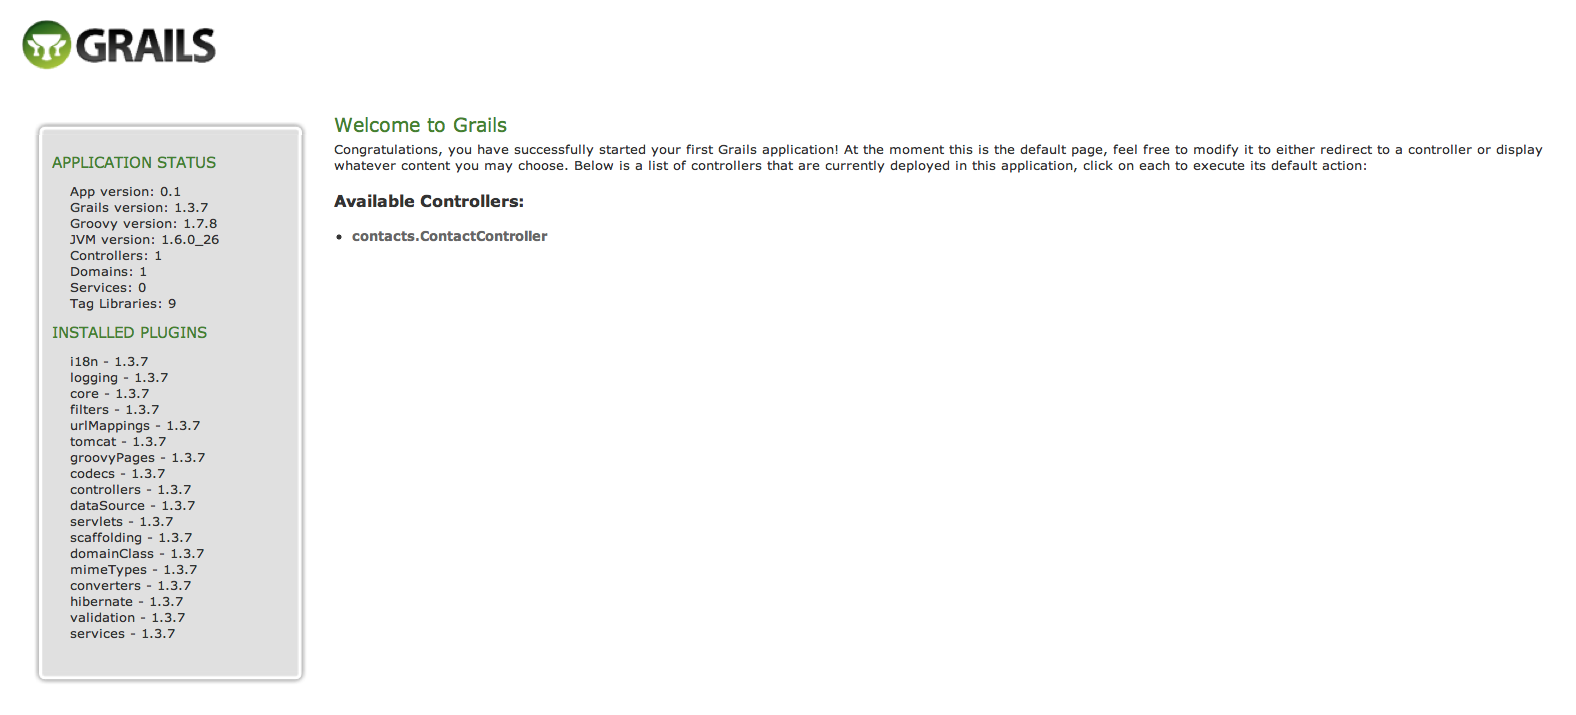
\includegraphics[width=.7\textwidth]{images/contactControllerScaffold.png}
       \caption{Controller de Contatos}
       \label{fig:contactScaffold1}
   \end{figure}
   
   Ao clicar em \emph{agenda.ContatoController} a aplicação redireciona o usuário para
   a página gerada pelo scaffold, como pode-se ver na figura \ref{fig:contactScaffold2}.
   
   \begin{figure}[h!]
      \centering
      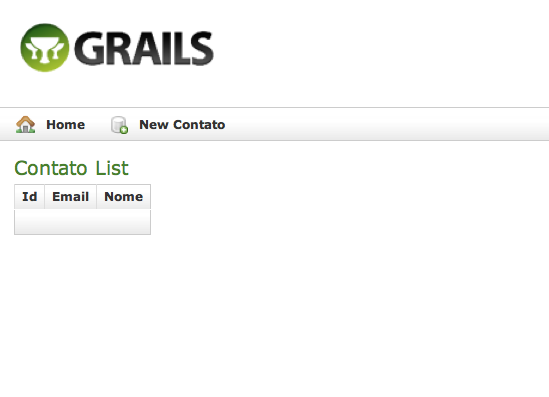
\includegraphics[width=.4\textwidth]{images/contactControllerScaffold2.png}
      \caption{Scaffolding de Contatos}
      \label{fig:contactScaffold2}
  \end{figure}
  
  Nessa página é possível disparar a criação de novos contatos e ver uma listagem
  dos contatos existentes. Como nesse momento não existe nenhum cadastrado a listagem
  não apresenta nenhum valor. A figura \ref{fig:createContactScaffold} mostra a 
  página gerada dinamicamente pelo scaffold que permite a criação de novos \textbf{contatos}.
  
   \begin{figure}[h!]
      \centering
      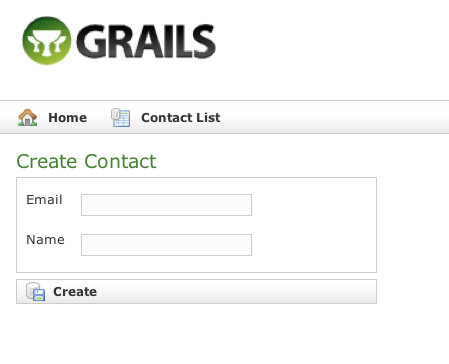
\includegraphics[width=.4\textwidth]{images/createContactScaffold.png}
      \caption{Página de criação de novos contatos gerada dinamicamente pelo scaffold}
      \label{fig:createContactScaffold}
  \end{figure}
  
  Após a criação do registro é exibida a página de exibição de contatos como pode 
  ser observado na figura \ref{fig:showContactScaffold} e na página de listagem
  agora o registro recém criado já pode ser visto, como na figura \ref{fig:listContactScaffold}.

   \begin{figure}[h!]
      \centering
      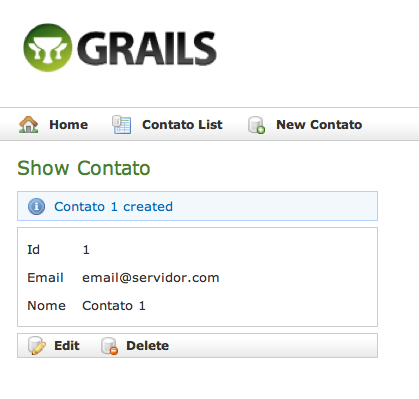
\includegraphics[width=.3\textwidth]{images/showContactScaffold.png}
      \caption{Página de exibição de um Contato gerada dinamicamente pelo scaffold}
      \label{fig:showContactScaffold}
  \end{figure}
  
   \begin{figure}[h!]
      \centering
      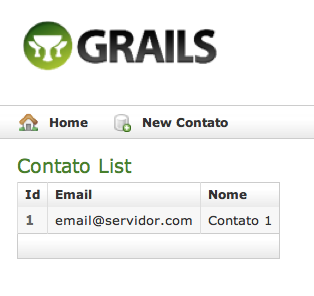
\includegraphics[width=.3\textwidth]{images/listContactScaffold.png}
      \caption{Página de exibição dos Contatos cadastrados gerada dinamicamente pelo scaffold}
      \label{fig:listContactScaffold}
  \end{figure}
  
\subsection{Complementando o modelo da aplicação}

  Para complementar as funcionalidades necessárias da aplicação será necessário 
  criar novas \emph{Domain Classes} e gerar os respectivos \emph{Controllers}. 
  Assim, vamos criar as \emph{Domain Classes} \texttt{Grupo} e \texttt{PropriedadeContato}.
  A classe \texttt{Grupo} representa o que o nome já deixa claro. Enquanto que a classe
  \texttt{PropriedadeContato} representa o conceito de propriedades dinâmicas para
  o nosso \texttt{Contato}. Assim, é possível criar diversos tipos de propriedades 
  para cada contato, e além disso, é possível que contatos distintos te\-nham propriedades
  distintas além do nome e email. A listagem \ref{GrupoV1} mostra a \emph{Domain Class}
  \texttt{Grupo} e a listagem \ref{GrupoControllerV1} o seu respectivo \emph{Controller}. 
  
  \lstinputlisting[
                    style=Groovy,
                    caption=Domain Class Grupo com propriedades name,
                    label=GrupoV1
                  ]
                  {src/groovy/agenda/grupo/GrupoV1.groovy}
 
  \lstinputlisting[
                    style=Groovy,
                    caption=Controller de Grupos,
                    label=GrupoControllerV1
                  ]
                  {src/groovy/agenda/grupo/GrupoControllerV1.groovy}
 
  A listagem \ref{GrupoV1} exibe uma novidade, requisitos de validação estão inseridos
  na classe através da \texttt{closure} estática \textbf{constraints}.
  Nela estão definidas duas validações para a propriedade \textbf{nome}. A primeira
  validação diz que nome não pode ser vazio. A segunda diz que nome não pode ser
  nulo. Estas restrições serão analisadas sempre que o método \texttt{validate()} 
  for invocado. Isto ocorre, por exemplo, sempre que o método \texttt{save} for 
  invocado. A figura \ref{fig:ValidacaoGrupo} mostra o resultado da validação da 
  tentativa de criação de um grupo sem nome.
  
  \begin{figure}[h!]
       \centering
       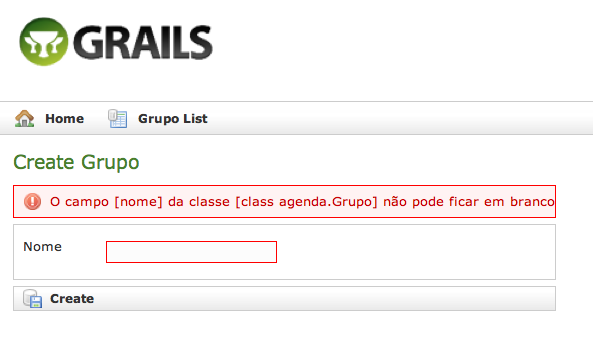
\includegraphics[width=.4\textwidth]{images/validacaoGrupo.png}
       \caption{Tentativa de criação de um grupo sem nome}
       \label{fig:ValidacaoGrupo}
   \end{figure} 
  
  A tabela \ref{tab:Validadores} ilustra as possíveis validações nativas no 
  framework segundo \cite{pragmaticGrails:2009}.

  \begin{table}[h!]
        \centering
        \caption{Validadores nativos do Grails}
        \label{tab:Validadores}
        \begin{tabular}{| l | c | l |}
        \hline
        {\bf Validador} & {\bf Parâmetros} & {\bf Descrição} \\
        \hline
            \texttt{blank} & \textbf{Boolean} & Permite que um valor seja uma string vazia \\
        \hline
            \texttt{nullable} & \textbf{Boolean} & Permite valores nulos \\
        \hline
            \texttt{max} & \textbf{Integer}  & Valor máximo \\
        \hline
            \texttt{min} & \textbf{Integer} & Valor mínimo \\
        \hline
            \texttt{size} & \textbf{Range} &  Determina os extremos \\
        \hline
            \texttt{maxSize}  & \textbf{Integer} & O tamanho máximo de uma String ou Collection \\
        \hline
            \texttt{minSize} & \textbf{Integer} & O tamanho mínimo de uma String ou Collection \\
        \hline
            \texttt{inList} & \textbf{List} & Lista de valores válidos \\ 
        \hline
            \texttt{matches} & \textbf{String} &  O valor deve ser reconhecido por uma expressão regular \\
        \hline
            \texttt{unique} & \textbf{Boolean} &  Reforça a unicidade do valor no Banco de Dados \\
        \hline
            \texttt{url} & \textbf{Boolean} & O valor deve ser uma URL válida \\
        \hline
            \texttt{email} & \textbf{Boolean} & O valor deve ser um email válido \\
        \hline
            \texttt{creditCard} & \textbf{Boolean} & O valor deve ser um número válido de cartão de crédito \\
        \hline
            \texttt{validator} & \textbf{Closure} & Recebe uma closure com dois parâmetros, o primeiro sendo \\
                               &                  & o valor e o segundo (opcional) a instância sendo validada \\
        \hline
        \end{tabular}  
    \end{table}
  
  Além de efetuar validação a \texttt{closure constraint} serve para orientar o \emph{scaffolding}.
  Customizações básicas podem ser criadas apenas alterando essa \texttt{closure}. As listagens
  \ref{PropriedadeContatoV1} e \ref{ContatoV2} exibem respectivamente as classes
  \texttt{PropriedadeContato} e a classe \texttt{Contato} atualizada com as validações.
  
  \lstinputlisting[
                      style=Groovy,
                      caption=Domain Class PropriedadeContato,
                      label=PropriedadeContatoV1
                    ]
                    {src/groovy/agenda/propriedades/PropriedadeContatoV1.groovy}
                    
  \lstinputlisting[
                    style=Groovy,
                    caption=Domain Class Contato atualizada com validações,
                    label=ContatoV2
                  ]
                  {src/groovy/agenda/contato/ContatoV2.groovy}
    
\subsection{Relacionamentos entre classes}
    
    Seguindo o fluxo de desenvolvimento da aplicação iremos agora tratar dos relacionamentos
    entre as classes criadas até o momento. Para a agenda, é claro que 1 \texttt{Grupo}
    possui várias referências à \texttt{Contatos} e que cada \texttt{Contato} pode
    ter várias propriedades além de \textbf{nome} e \textbf{email}. Para criar 
    relacionamentos entre as classes o framework apresenta o \textbf{GORM}. Uma 
    abstração acima do Hibernate e que pode ser facilmente configurado.
    
    Propriedades simples e relacionamentos \textbf{1 para 1} podem ser configurados
    apenas utilizando o mecanismo de validação em conjunto com a definição do tipo.
    Esta é a razão pela qual as propriedades das \emph{Domain Classes} criadas até o momento
    utilizam tipos em vez da palavra chave \texttt{def}, o que seria perfeitamente
    possível.
    
    Relacionamentos \textbf{1 para muitos} como no caso entre \texttt{Grupo} e \texttt{Contato} são
    configurados utilizando uma propriedade estática chamada \texttt{hasMany}. As chaves
    do mapa representam o nome das propriedades na classe que detém o relacionamento
    e os valores são os tipos dos objetos do relacionamento. A listagem \ref{GrupoV2}
    mostra o relacionamento entre um \texttt{Grupo} e seus diversos \texttt{Contatos}.
    
    \lstinputlisting[
                      style=Groovy,
                      caption=Relacionamento entre Grupo e os seus Contatos,
                      label=GrupoV2
                    ]
                    {src/groovy/agenda/grupo/GrupoV2.groovy}
    
    A \texttt{closure hasMany} recebe um mapa contendo o nome das propriedades e seus respectivos
    tipos. A leitura fluída permite quase que uma tradução direta de que um \texttt{Grupo}
    possui muitos \texttt{Contatos}. O mesmo se aplica para as propriedades dos contatos, 
    como pode ser visto na listagem \ref{ContatoV3}.
    
    \lstinputlisting[
                      style=Groovy,
                      caption=Relacionamento entre Contato e as suas Propriedades,
                      label=ContatoV3
                    ]
                    {src/groovy/agenda/contato/ContatoV3.groovy}
    
    Para relacionamentos \textbf{muitos-para-muitos} usa-se a \texttt{closure hasMany} e a 
    propriedade \texttt{belongsTo} que representa o lado que detém a posse do relacionamento.
    

\subsection{Materializando Controllers e Views}
    
    Até o presente momento, todo o código escrito se encontra nas \emph{Domain Classes}.
    Os \emph{Controllers} utilizam \emph{scaffolding} e não existe código de \emph{View}. Para implementar
    as funcionalidades restantes do projeto se faz necessário alterar o código dos
    \emph{Controllers}. Para isso, o seguinte comando deve ser executado:
    
    \begin{lstlisting}[basicstyle={\small \ttfamily}]
           grails generate-all "*"
    \end{lstlisting}
    
    Isso irá fazer com que o código dinamicamente gerado do \emph{scaffolding} seja "materializado"
    nos \emph{Controllers} permitindo assim, que seja modificado. O resultado final pode
    ser visto na listagem \ref{ContatoControllerV3}.
    
    \lstinputlisting[
                     style=Groovy,
                     caption=ContatoContoller gerado,
                     label=ContatoControllerV3
                   ]
                   {src/groovy/agenda/contato/ContatoControllerV3.groovy}
    
    De maneira semelhante, o \emph{Controller} de \texttt{Grupos} possui os mesmos métodos. 
    Cada \emph{action} possui uma  \emph{View} associada. A listagem \ref{ContatoCreateView} 
    exibe a \emph{View} associada à \texttt{action create}.
    
    \lstinputlisting[
                     style=JAVA,
                     caption=View da action create,
                     label=ContatoCreateView,
                     basicstyle=\small
                   ]
                   {src/groovy/agenda/contato/createV1.gsp}
    
\subsection{Associando Contatos a Grupos}

    Para associar um \textbf{contato} a um \textbf{grupo} deve-se alterar o \emph{Controller}
    \texttt{GrupoController} criando uma \emph{action} responsável para a tarefa.
    A listagem \ref{GrupoControllerV4} mostra o código da action recém criada.
    
    \lstinputlisting[
                     style=groovy,
                     caption=Action associarContato,
                     label=GrupoControllerV4
                   ]
                   {src/groovy/agenda/grupo/GrupoControllerV4.groovy}
    
    As linhas 2 e 3 respectivamente, capturam dos parâmetros enviados para a action
    os id do contato e do grupo e carregam na memória os objetos correspondentes.
    A linha 5 testa a existência do grupo selecionado, na linha 6 ocorre a checagem
    através do relacionamento entre grupo e contato se o contato selecionado já está
    associado ao grupo. Em caso positivo, o contato é desassociado do grupo, caso
    contrário, ele é associado ao grupo. A linha 14 por sua vez, encerra a requisição
    e retorna o status http 200 que significa sucesso.
    
    Para a utilização dessa action se faz necessário alterar o arquivo que da view
    responsável pela edição. 

\subsection{Groovy Server Pages}

    A tecnologia utilizada para renderização das views é o framework Groovy Server 
    Pages, GSP. Similar ao Java Server Pages, o GSP permite a criação de dinâmica 
    de conteúdo misturando conteúdo estático e dinâmico através de tags html e da
    biblioteca de tags embutidas as taglibs. É possível ainda criar as próprias tags
    customizadas.
    
    Para a action desenvolvida na seção anterior não será criada nenhuma taglib 
    customizada, mas serão usadas algumas taglibs do framework. A listagem \ref{associarContatoViewV1}
    mostra o trecho de código alterado na view de edição de grupos.
    
    \lstinputlisting[
                     style=java,
                     caption=Trecho de código da view de edição de grupos responsável por associar contatos,
                     label=associarContatoViewV1
                   ]
                   {src/groovy/agenda/grupo/associarContatoViewV1.gsp}
    
    Em resumo, esse trecho de código é composto pela listagem de todos os
    contatos cadastrados. Cada um com \emph{checkbox} representando a existência 
    ou ausência do relacionamento entre ele e grupo atualmente sendo editado 
    de acordo com o estado da seleção.

    Na linha 4 se vê a utilização da \texttt{taglib} \texttt{message} responsável por exibir
    mensagens de texto retiradas dos arquivos de internacionalização disponíveis 
    na pasta \emph{grails-app/i18n}. A linha 12 exibe uma forma de iteração nos 
    itens de uma coleção através da \emph{tag} \texttt{each}. Uma referência completa 
    sobre as \emph{tags} \texttt{gsp} pode ser encontrada na página \url{http://grails.org/doc/latest/guide/single.html#6.2.2 GSP Tags}. 
    
    Um detalhe a ser notado está na linha 16, uma associação do evento de clique 
    no \emph{checkbox} a uma função \texttt{javascript}, responsável por executar 
    uma chamada à \emph{action} \texttt{associarContato} do \texttt{GrupoController}.
    A listagem \ref{associarContatoScriptV1} exibe o trecho com o script necessário
    ao funcionamento do código.
    
    \lstinputlisting[
                     style=java,
                     caption=Javascript de chamada à action associarContato do GrupoController,
                     label=associarContatoScriptV1
                   ]
                   {src/groovy/agenda/grupo/associarContatoScriptV1.js}
    
    Por questões de visualização a chamada na linha 3 foi quebrada em mais de uma linha. 
    O funcionamento básico da chamada é executar uma requisição http utilizando o método
    \texttt{POST} para a \emph{url} \url{associarContato} que é relativa ao \emph{path} 
    atual. O resultado é que ao executar este método a \emph{action} \texttt{associarContato} 
    vai ser executada e ao final o contato vai estar associado ao grupo ou removido dele.   
    
\subsection{Instalando Plugins}

    A arquitetura do framework permite a criação e instalação de plugins permitindo assim,
    que novas funcionalidades sejam agregadas sem alterar o código original. Para executar
    a tarefa da seção anterior foi instalado o \emph{plugin jquery}. O plugin permite a 
    utilização do \emph{jQuery} nos projetos \emph{Grails}.
    
    O jQuery é um framework javascript também muito customizável e bastante difundido.
    Para a instalação do plugin é preciso executar o comando:
    
    \begin{lstlisting}[basicstyle={\small \ttfamily}]
           grails install-plugin jquery
    \end{lstlisting}
    
    Automáticamente o Grails irá criar toda a infraestrutura necessária para a utilização
    do plugin. No caso específico do plugin jquery existe ainda um passo a ser executado.
    Adicionar a seguinte linha ao final da seção \emph{head} arquivo \emph{grais-app/views/main.gsp}
    
    \begin{lstlisting}[style=Java]
            <g:javascript library="jquery" plugin="jquery"/>
    \end{lstlisting}

    %iniciar uma subseção e falar sobre o grails
    %incluir:
    %   introdução ao grails -> DONE
    %   instalação -> DONE
    %   descrição da aplicação (Google Contacts Clone) -> DONE
    %   script de criação da aplicação -> DONE
    %   convention-over-configuration -> DONE
    %   domain classes -> DONE
    %   controllers -> DONE
    %   scaffolding -> DONE
    %   validação -> DONE
    %   GORM
    %       - Relacionamentos:
    %           1-para-1 -> DONE
    %           1-para-muitos -> DONE
    %           muitos-para-muitos -> DONE
    %       - Finders
    %           
    %   views -> DONE
    %       GSP -> DONE
    %   plugins -> DONE
    %\section{Figures and Captions}\label{sec:figs}

    
\section{Conclusão}

    Desde seu surgimento, a plataforma Java se destaca como uma ótima alternativa
    para o desenvolvimento de aplicações \emph{web}. Diversos \emph{frameworks} surgiram para 
    proporcionar reutilização de código e aumento de produtividade. Apesar disto,
    outras tecnologias têm se destacado no cenário de desenvolvimento de software
    para a web. 
    
    A primeira parte deste artigo abordou os conceitos básicos da linguagem \texttt{Groovy} e
    do \emph{framework} \texttt{Grails} e como essas tecnologias podem ser utilizadas 
    para a criação de aplicações \emph{web} com pouco esforço. 
    
    Na segunda parte foram exibidas algumas características dinâmicas da linguagem 
    \texttt{Groovy}, sua redefinição de operadores, uso de coleções simplificado, definição
    de métodos e o conceito de closures.
    
    Por último, na terceira do artigo destacou-se o framework Grails e suas características
    principais, a criação de Domain Classes, a validação de propriedades, a criação de Controllers,
    a utilização de Scaffolding, os relacionamentos de entidades do domínio através do
    GORM, a criação de Views finalizando com a construção de uma chamada Ajax a uma action
    através da utilização de plugins. Todos os conceitos exibidos nessa parte do artigo
    possuem exemplos práticos através de uma aplicação que foi desenvolvida utilizando 
    as técnicas e os conceitos abordados anteriormente.
    
    Apesar de cobrir boa parte do \emph{framework}, ainda existem características que 
    merecem atenção. Devido ao escopo deste artigo estas não puderam ser abordadas. 
    Como forma de continuação dos estudos no assunto, sugere-se a análise de técnicas 
    como Desenvolvimento Orientado a Testes, \texttt{TDD}, devido à grande facilidade 
    e ao grande estímulo da comunidade de \emph{software}  e do \emph{framework} a esta
    técnica. Além disso, convém estudar a integração do \texttt{Grails} com  outros 
    \emph{frameworks} web. Algumas sugestões a seguir, \texttt{Spring Security} 
    (\url{http://static.springsource.org/spring-security/site/}), que provê características
    de segurança e o \texttt{Apache Solar} (\url{http://lucene.apache.org/solr/}) que 
    provê características de indexação e busca textual.
    
\bibliographystyle{sbc}
\bibliography{artigo}

\end{document}
